\section{Optimization with Graph Filtering}
\label{sec-opt}

In this section, we propose graph filtering based optimization techniques to
enhance the algorithm proposed in Section~\ref{sec-topk}.

Our optimization techniques works for the following scenario.
We have a local data graph $G$ and a user specified positive integer $r$, and
we want to find top-$k$ group recommendations for each {\em online query}
$\langle Q, k\rangle$, where $Q$ is a pattern graph and $k$ is a positive
integer, \ie find the top-$k$ densest valid groups for $Q$ of $G$ \wrt $r$ for
each online query $\langle Q,k\rangle$.

The optimization is based on an idea of graph filtering: filter out the candidates that are not possible to contain results as early as possible. After executing top-$k$ offline process and before executing top-$k$ online process, we can employ a filtering process on $BL$ to remove the balls that are not possible to contain valid groups, which we refer to as false balls. And that will certainly reduce the execution time in finding out top-$k$ results. It contains a filtering offline preprocessing process over the set of balls in $BL$, and a filtering online process for each input query, in which we utilize an effective and efficient pruning strategy to remove false balls from $BL$ as many as possible. Finally, we can execute top-$k$ online process on the revised ball list $BL$.

In filtering offline process, we need to identify some pruning rules, which is usually executed based on features selected from candidates. In filtering online process, given a query graph, if there exists a feature that the query graph has while a data ball does not have, the data ball will be eliminated from the candidate set safely. \textcolor[rgb]{0.00,0.00,1.00}{TO be more CONCRETE!}


\subsection{Offline(\&online): Building Hybrid Star-feature Indices}

\stitle{Star-feature selection}

When deal with directed graphs, as we have seen in section~\ref{subsec-extsim}, graph simulation preserves the labels and the child relationship of a graph pattern in its match. When it comes to undirected graphs, graph simulation still preserves the label relationship, and preserves the neighbor relationship of a graph pattern in its match instead of child relationship in directed graphs. Therefore, we utilize the ``neighbor relationship" character as the pruning rule, and use the feature ``star" to represent the ``neighbor relationship" character. A star is a graph structure with a center node in the middle and a set of neighbor nodes adjacent with the center node. For each ball $\ball{v, r}$ in data graph $G$, and for each node $w$ in the ball, we construct one corresponding star-feature, eg..., so we get a set of star-features $F$ for each ball.

For all the balls $\ball{v, r}[1]$, $\ball{v, r}[2]$,...,$\ball{v, r}[n]$ in data graph $G$, we construct the corresponding feature sets $F[1]$,$F[2]$,...,$F[n]$. When a pattern graph comes, we construct the corresponding star-feature set $FP$ and compare it with $F[i]$ ($1\leq i\leq n$) of $\ball{v, r}[i]$. For each feature $fp$ in $FP$, if there exists a feature $f$ in $F[i]$ containing $fp$ as a substructure, then there may exist a matching result in $\ball{v, r}[i]$ and need further validation in the top-$k$ process. Otherwise, $\ball{v, r}[i]$ is pruned from candidate set safely.

In the above indices construction, for each ball $\ball{v, r}[i]$ ($1\leq i\leq n$) with $m_i$ nodes, we construct $m_i$ star-features. But it may be a waste of time and space to retrieve and store such lots of features, we can retrieve less features with stronger filtering power, making a balance between complexity and the pruning power. Therefore, We will improve this by adopting the next two star-feature selection strategies respectively.

Given a graph $H$, we want to select as few star-features as possible, which requires each star-feature to have strong pruning power and differ from other star-features obviously. This inspires us to think about the star minimization problem we will discuss in this section.

\etitle{Star minimization problem}. Given a graph $H(V_h, E_h)$, Star minimization problem is to select a set of star-features $F$ from $H$, with the union of edges of star-features in $F$ covering all the edges in $E_h$, while $|F|$ is minimized.

\begin{theorem}
\label{thm-star-mini-complexity}
Given a graph $H(V_h, E_h)$, and a positive integer $\xi$, it is \NP-complete to determine whether there exists a star-feature set $F$ with the union of edges of star-features in it covering all the edges in $E_h$, and the number of items in $F$ is no larger than $\xi$.
\end{theorem}

\textbf{Approximation hardness:}

\begin{theorem}
\label{thm-star-mini-complexity}
There exists a factor 2 approximation algorithm for the Star minimization problem.
\end{theorem}

We present the 2-approximation algorithm in Fig.~\ref{star-min-alg}.

\begin{figure}[tb!]
\vspace{2ex}
\begin{center}
{\small

\myhrule \vspace{-2ex}
\mat{0ex}{
\sstab {\sl Input:\/} Graph $H(V_h$, $E_h)$.\\
{\sl Output:\/} The set of star-feature $F$ of $H$.\\
\bcc \quad $C:=\emptyset$; $F:=\emptyset$;\\
\icc \quad $H'(V_h', E_h'):=H(V_h, E_h)$;\\
\icc \quad while $E_h'$ is not empty do\\
\icc \quad\quad pick any $(u, v) \in E_h'$;\\
\icc \quad\quad $C:=C \cup \{(u, v)\}$;\\
\icc \quad\quad remove all edges incident to either $u$ or $v$ in $H'$.\\
\icc \quad for each node $w$ in $C$ do\\
\icc \quad\quad construct star feature $f$ takes $w$ as the center node in $H$;\\
\icc \quad\quad $F:=F \cup f$;\\
\icc return $F$;\\

}
\vspace{-2.5ex} \myhrule
}
\end{center}
\vspace{-4ex}
\caption{Algorithm StarMin} \label{star-min-alg}
\vspace{-3ex}
\end{figure}

There is another scene that users have the chance to specify a number, indicating how many star-features necessarily to be selected from the given graph. It requires the fixed number of star-features we select should have strong pruning power, representing as much structural information as possible. This is another feature selection strategy we will consider next.

\etitle{$K$-star coverage maximization problem}. Given a graph $H(V_h, E_h)$ and a user specified integer $K$, $K$-star coverage maximization problem is to select a set of star-features $F$ from $H$, with the union of edges of star-features in $F$ covering as many edges as possible in $E_h$.

\begin{theorem}
\label{thm-k-star-max-complexity}
Given a graph $H(V_h, E_h)$, two positive integers $K$ and $\xi$, it is \NP-complete to determine whether there exists a $K$ item star-feature set $F$, in which the number of the union of edges of the star-features is no smaller than $\xi$.
\end{theorem}

\textbf{Approximation hardness:}

\begin{theorem}
\label{thm-star-mini-complexity}
There exists a 3/4-approximation algorithm for the $K$-star coverage maximization problem.
\end{theorem}

We present the 3/4-approximation algorithm in Fig.~\ref{k-star-max-alg}.

\begin{figure}[tb!]
\vspace{2ex}
\begin{center}
{\small

\myhrule \vspace{-2ex}
\mat{0ex}{
\sstab {\sl Input:\/} Graph $H(V_h$, $E_h)$, a positive integer $K$.\\
{\sl Output:\/} The set of star-feature $F$ of $H$.\\
\bcc \quad $C:=\emptyset$; $F:=\emptyset$;\\
\icc \quad for $i=1$ to $K$ do\\
\icc \quad\quad select node $v$ from $H$ while the number of edges $C \cup \{v\}$ \\covers is maximized ;\\
\icc \quad for each node $w$ in $C$ do\\
\icc \quad\quad construct star feature $f$ takes $w$ as the center node in $H$;\\
\icc \quad\quad $F:=F \cup f$;\\
\icc return $F$;\\

}
\vspace{-2.5ex} \myhrule
}
\end{center}
\vspace{-4ex}
\caption{Algorithm K-StarMax} \label{k-star-max-alg}
\vspace{-3ex}
\end{figure}

\textcolor[rgb]{1.00,0.00,0.00}{\textbf{Remark.}
Establish the filtering power standards of star features.
1. Covering more edges
2. Covering more nodes}

\stitle{Hybrid Star Index Structure}.

In last section, for each ball $\ball{v, r}$ in data graph $G$, we construct a star-feature set $F$. When a pattern graph $P$ comes, we construct the corresponding star-feature set $FP$ and compare it with $F$. If $P$ and $\ball{v, r}$ are matched via extended graph simulation, for each star-feature $fp$ in $FP$, there must exist a corresponding $f$ in $F$ such that $fp$ is a substructure of $f$. That is, the local structure represented by $fp$ in $P$ must be preserved by $f$ in $\ball{v, r}$. Therefore, we need to check all the star-features in $FP$ to see whether there exist the corresponding structures in $\ball{v, r}$ preserving the local structure, such that we can remove the false positives in the filtering process. However, a question arises, as the structure comparison operation is expensive, how can we implement the checking process efficiently? In this section, we propose Hybrid-Star-Index-Structure to encode the local information of star-features selected in last step, improving the speed of comparison operation in filtering process to a large extent.

\etitle{Index structure for small label data graph}

We will present a encoding method, for the case when the number of labels appearing in data graph is small, which encodes the local information taken by the star to numerical space. For each star-feature, it generates a bit string with fixed-length, called \textbf{Star-fingerprint}, providing a convenient way to execute filtering process just on those star fingerprints, with no need referring to the originally star-feature structures.

\begin{definition} {\textbf{Star-fingerprint.}}
\label{def-ind-str-small-label}
Given a data ball $\ball{v, r}$ in $G$ and the corresponding star-feature set $F=\{s_1, s_2,..., s_m\}$ of the ball, for any star-feature $s_i$ $(1 \leq i \leq m)$ in $F$, the star-fingerprint $starfig(s_i)$ of $s_i$ is a two-tuples $<C,N>$, where $C$ denotes the center node with id and label of star $s_i$, and $N$ is a length-$L$ bit string, denoting the neighbor labels, where $L$ is the total number of labels appearing in $G$, and each bit indicates the appearance of the corresponding label in neighbors.
\end{definition}

By Definition~\ref{def-ind-str-small-label}, in the two-tuples $<C,N>$, $C$ is to denote the center node and $N$ is to denote the neighbor labels of center node. For each distinct neighbor label, it sets the corresponding position element in the bit string to 1, indicating there exists at least one neighbor node carrying the label. For example, Fig~\ref{fig-starfingerprint-example} shows an example on how to generate the star-fingerprint.

\begin{figure}[tb!]
\begin{center}
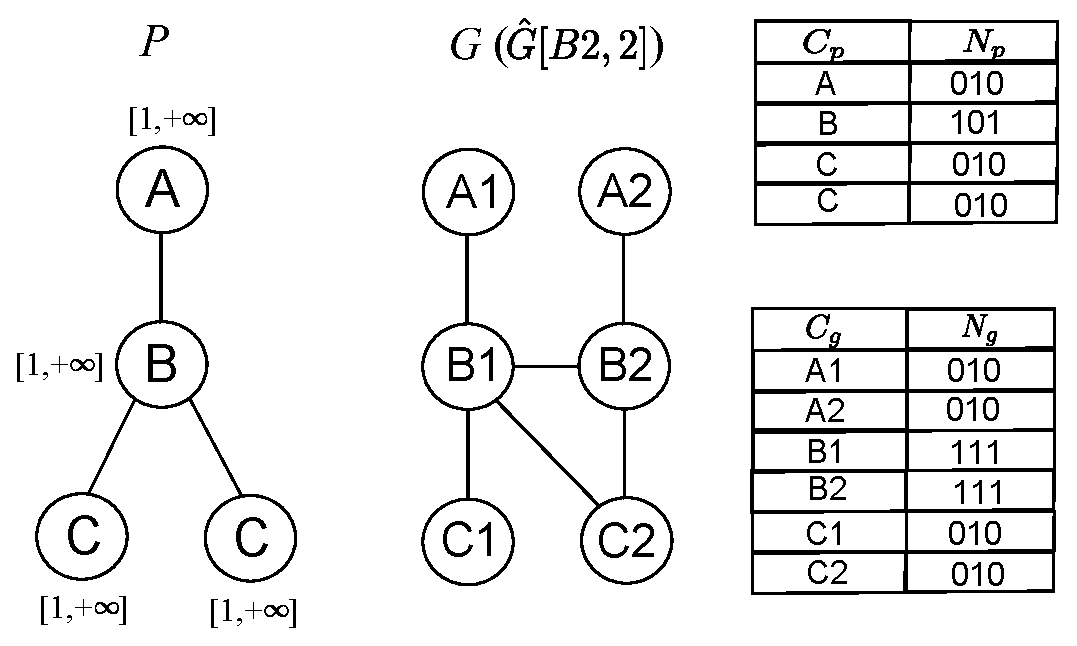
\includegraphics[scale=0.4]{./fig/star-fingerprint.eps}
\caption{Star Fingerprint}
\label{fig-starfingerprint-example}
\end{center}
\end{figure}


\begin{prop}
\label{prop-star-fingerprint-condition}
Given a data graph $G$, a pattern graph $P$, and a positive integer $r$, if subgraph $G_{s}$ of $G$ is a {\em valid group} for $P$ \wrt $r$, then for each vertex $v$ in $P$, whose star-feature is $s_v$, and star-fingerprint $starfig(s_v)$ is $<C_p,N_p>$, there must exist a matched vertex $u$ in $G_{s}$, whose star-feature is $s_u$, and star-fingerprint $starfig(s_u)$ is $<C_g,N_g>$. The two star fingerprints must satisfy the following two conditions: 1)$l(C_p)=l(C_g)$; 2)$N_p \wedge N_g = N_p$.
\end{prop}

By proposition~\ref{prop-star-fingerprint-condition}, assume $G_{s}$ of $G$ is a {\em valid group} of $G$ for $P$. A vertex $v$ in $P$ is matched with a vertex $u$ in $G_{s}$. The vertices $v$ and $u$ are matched via extended graph simulation requires the two conditions hold, because according to extended graph simulation, the labels of $v$ and $u$ must be same (condition 1); and the labels of neighbors of $v$ must be a subset of the labels of neighbors of $u$ (condition 2).

\begin{theorem} {\textbf{Star-fingerprint Pruning 1.}}
\label{thm-star-fingerprint-pruning}
Given a data ball $\ball{v, r}$ of $G$ and a pattern graph $P$, for each vertex $v$ in $P$ with star-feature $s_v$, if there exists no vertex $u$ in $\ball{v, r}$ with star-feature $s_u$, where fingerprints $starfig(s_v)$ and $starfig(s_u)$ satisfy the two conditions in proposition~\ref{prop-star-fingerprint-condition}, there must exist no {\em valid group} in $\ball{v, r}$ of $G$ for $P$.
\end{theorem}

Apparently, this is a feature to feature comparison, and we can prune the set of balls cannot have a valid group inside quickly according to the pruning rule proposed in  theorem~\ref{thm-star-fingerprint-pruning}. It has a good performance when the length-$L$ bit string is short, as the comparison between two fingerprints can be executed by a bitwise AND operation in $O(L)$ time.

\etitle{Index structure for large label data graph}

When the number of labels appearing in data graph is really large, it is inconvenient to adopt the star-fingerprint method to represent the star feature. That is, when $L$ is large, adopting the $L$-length bit string is not efficient for the star feature expression and feature to feature comparison. Therefore, we will present another encoding method for representing star-features extracted from the data graph with large number of labels. For each star-feature, it generates a bit string with specified length, called \textbf{Star-bloomfilter}. This is a method based on the space-efficient data structure \textbf{bloom filter}, both reducing the storage space requirement and improving filtering speed.

A Bloom filter is a length-$X$ bit string. Given a set of elements and a query item, the bloom filter is used to check whether the query element is contained in the set. There are also $k$ predefined hash functions, each of which hashes an item to one of the $X$ positions with a uniform random distribution. For each element, feed it to each of the $k$ hash functions to get $k$ bit positions, and set the bits at all these positions to 1. To query whether there exists an element in the set, just feed it to each of the $k$ hash functions to get $k$ bit positions, check whether all these bits are set to 1. If there exists any position the bit is 0, then the element is not in the set. If it were, then the element has a high probability in the set, but there may exist ``false positives" due to collisions in hash functions. By this observation, given a query graph and a data ball, when executing the feature to feature comparison, say $f$ in data ball and $fp$ in query graph, we can use a bloom filter to encode the neighbor label set of $s$, and check for each neighbor label in $fp$, whether it is contained in $s$ by checking the bloom filter. Finally, we can filter out a set of unmatched data balls in advance.

\begin{definition} {\textbf{Star-bloomfilter.}}
\label{def-ind-str-large-label}
Given a data ball $\ball{v, r}$ in $G$ and the corresponding star-feature set $F=\{s_1, s_1,..., s_m\}$  of the ball, for each star-feature $s_i$ $(1 \leq i \leq m)$ in $F$, the star-bloomfilter $starblm(s_i)$ of $s_i$ is a two-tuples $<C,N>$, where $C$ denotes the center node with id and label of star $s_i$, and $N$ is a length-$X$ bit string bloom filter, denoting the neighbor labels, where $X$ is a user specified number.
\end{definition}

By Definition~\ref{def-ind-str-large-label}, in the two-tuples $<C,N>$, $C$ is to denote the center node and $N$ is to denote the neighbor labels of center node. For each distinct neighbor label, by the set of $k$ hash functions, it sets the corresponding $k$ position element in the bit string to 1, indicating there exists at least one neighbor node carrying the label. For example, Fig~\ref{fig-bloomfilter-example} shows an example on how to generate the star-bloomfilter.

\begin{figure}[tb!]
\begin{center}
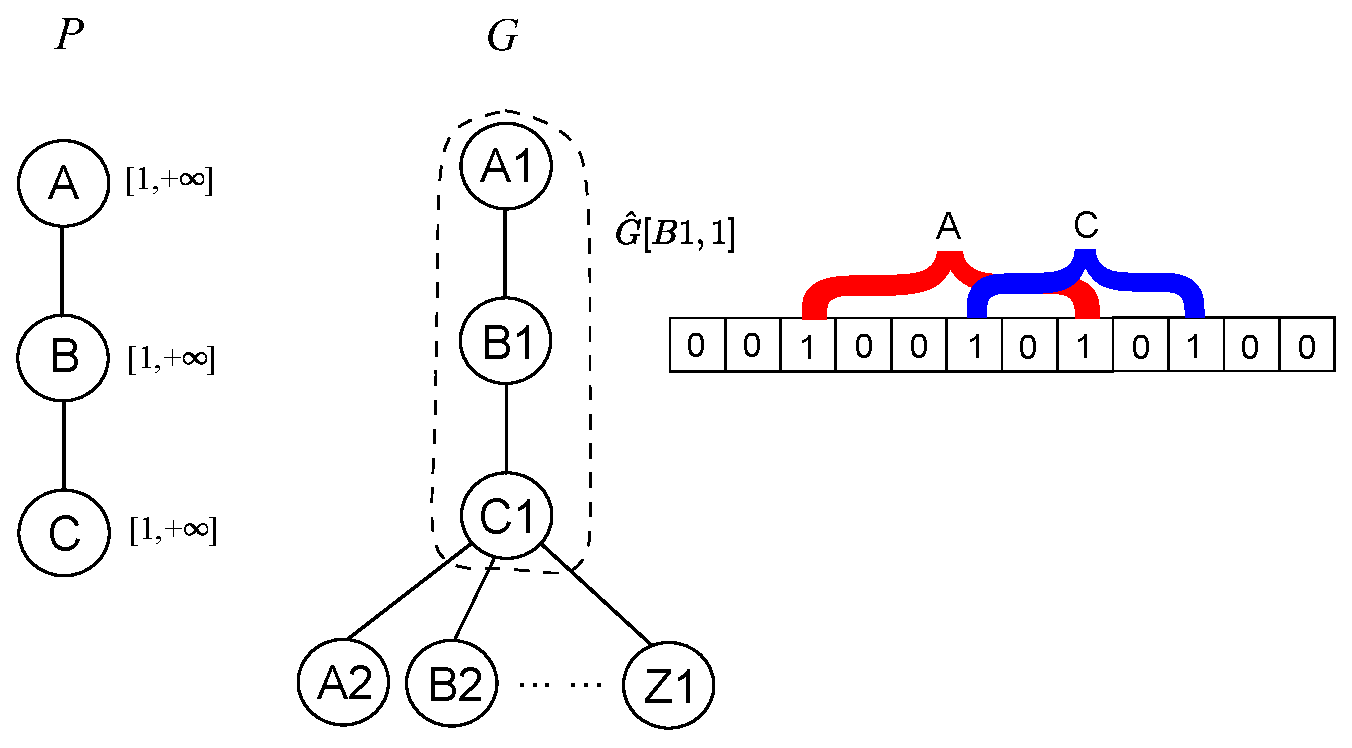
\includegraphics[scale=0.4]{./fig/star-bloomfilter.eps}
\caption{Star Bloomfilter}
\label{fig-bloomfilter-example}
\end{center}
\end{figure}


\begin{prop}
\label{prop-star-bloomfilter-condition}
Given a databall graph $G$, a pattern graph $P$, and a positive integer $r$, if subgraph $G_{s}$ of $G$ is a {\em valid group} for $P$ \wrt $r$. Then for each vertex $v$ in $P$, whose neighbor label set is $lset$, there must exists a matched vertex $u$ in $G_{s}$, whose star-feature is $s_u$, and star-bloomfilter $starblm(s_u)$ is $<C_g,N_g>$. They must satisfy the following two conditions: 1)$l(v)=l(C_g)$; 2)for each item in $lset$, feed it to each of the $k$ hash functions to get $k$ bit positions in $N_g$, all the $k$ bits are set to 1.
\end{prop}

By proposition~\ref{prop-star-bloomfilter-condition}, assume $G_{s}$ of $G$ is a {\em valid group} of $G$ for $P$. A vertex $v$ in $P$ is matched with a vertex $u$ in $G_{s}$. The vertices $v$ and $u$ are matched via extended graph simulation requires the two conditions hold, because according to extended graph simulation, the labels of $v$ and $u$ must be same (condition 1); and the labels of neighbors of $v$ must be a subset of the labels of neighbors of $u$ (condition 2).

\begin{theorem} {\textbf{Star-bloomfilter Pruning 2.}}
\label{thm-star-bloomfilter-pruning}
Given a data ball $\ball{v, r}$ of $G$ and a pattern graph $P$, for a vertex $v$ in $P$, if there exists no vertex $u$ in $\ball{v, r}$ with star-feature $s_u$, where $v$ and bloomfilter $starblm(s_u)$ of $u$ satisfy the two conditions in proposition~\ref{prop-star-bloomfilter-condition}, there must exist no {\em valid group} in $\ball{v, r}$ of $G$ for $P$.
\end{theorem}

Obviously, when the label number $L$ is small, we can use the length-$L$ star-fingerprint bit string, in which each bit represents a label directly; when the label number $L$ is large, we can reduce the storage space of a star feature encoding string significantly by utilizing bloomfilter data structure, from length-$L$ star-fingerprint bit string to length-$X$ star-bloomfilter bit string by using hash functions.

\textcolor[rgb]{1.00,0.00,0.00}{\textbf{Remark.}
Probability analyze for bloomfilter}

\stitle{Index structure for the whole data ball(Graph Code)}.

The above ``star to star" pruning process is time-consuming. We will next provide some quick pruning rules based on graph code. Such that when a query graph comes, we could execute ``graph to graph" filtering first, quickly pruning out the set of candidates obviously cannot match with query graph in the first filtering phase, and then employ the ``star to star" filtering with stronger pruning capability. We know that extended graph simulation preserves label and number relationship between data graph and pattern graph, so we can take those two characters as a pruning rule. In the first filtering phase, we could efficiently eliminate the set of candidates which violate the label and number constraints taken by pattern graph. Then in the second phase, we further check whether the candidates preserve the structural constraints taken by pattern graph by making the ``star to star" validation.

In this section we will present a encoding method for data balls, which encodes the label and node number information taken by the ball to numerical space. For each data ball, it generates a list , called \textbf{Graph-code}.

\begin{definition} {\textbf{Graph-code.}}
\label{def-ind-graph-code-arr}
Given a data ball $\ball{v, r}$ of $G$, the graph-code $B$ of $\hat{G}$ is a list. Each item in the list is a two-tuple $<Lab, Num>$, where $Lab$ indicates there exists at least one node in $\hat{G}$ labeled with $Lab$, and $Num$ denotes there are $Num$ nodes carrying the label $Lab$.
\end{definition}

Fig.~\ref{fig-graphcode-example} shows an example on how to generate the Graph code. \textcolor[rgb]{0.00,0.00,1.00}{MORE examples, combine with star-feature.}

\begin{figure}[tb!]
\begin{center}
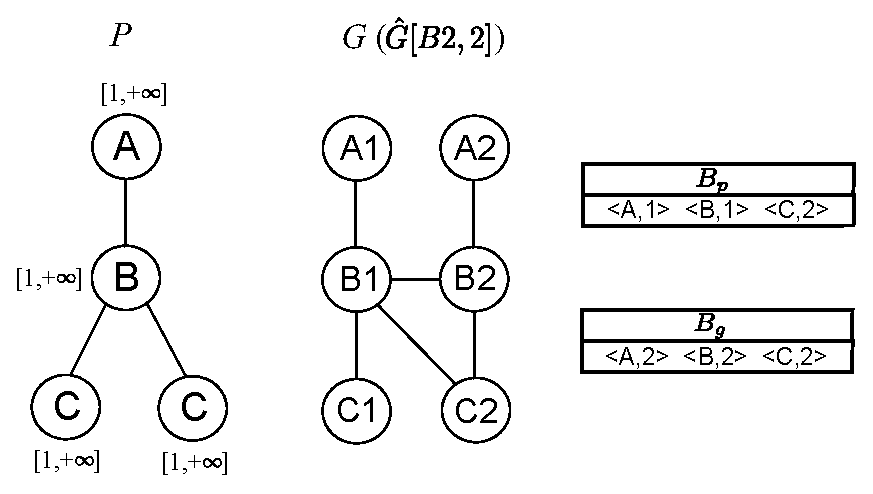
\includegraphics[scale=0.5]{./fig/graph-code.eps}
\caption{Graph Code}
\label{fig-graphcode-example}
\end{center}
\end{figure}

\begin{prop}
\label{prop-graph-code-condition}
Given a data graph $G$, a pattern graph $P$, and a positive integer $r$, if subgraph $G_{s}$ of $G$ is a {\em valid group} for $P$ \wrt $r$, and is contained in $\ball{v, r}$. The graph code $B_p$ of $P$ and the graph code $B_g$ of $\ball{v, r}$ must satisfy the following conditions:  for each item $<Lab_p,Num_p>$ in $B_p$, there must exist the corresponding item $<Lab_g,Num_g>$ in $B_g$ with 1) $Lab_p=Lab_g$, and 2) $Num_p \leq Num_g$.
\end{prop}

By proposition~\ref{prop-graph-code-condition}, assume $G_{s}$ of $G$ is a {\em valid group} of $G$ for $P$, and is contained in $\ball{v, r}$. $P$ and $G_{s}$ in $\ball{v, r}$ match via extended graph simulation requires the above conditions hold. Because according to extended graph simulation, each label $l$ contained in $P$ must be contained in $\ball{v, r}$, and the number of nodes labeled with $l$ must satisfy the lower bound requirement in $P$.

\begin{theorem} {\textbf{Graph-code Pruning 3.}}
\label{thm-graph-code-pruning}
Given a data ball $\ball{v, r}$ of $G$ and a pattern graph $P$, if there exists no subgraph $G_s$ in $\ball{v, r}$, where graph-code $B_p$ of $P$ and $B_g$ of $\ball{v, r}$ satisfy the conditions in proposition~\ref{prop-graph-code-condition}, there must exist no {\em valid group} in $\ball{v, r}$ for $P$.
\end{theorem}

Apparently, this is a graph to graph comparison, and we can efficiently prune out the set of candidates which violate the label and number constraints taken by pattern graph. It has a good performance as the comparison between two lists can be executed by linear scanning operation in $O(l_p+l_g)$ time ($l_p$ is the number of labels in $P$, and $l_g$ is the average number of labels among all the balls? Does average work?).

\subsection{(Online:) Improving Early Termination}

In order to accelerate the speed of finding match results, we combine the top-k early termination process with filtering method. Given a data graph $G$, we first generate the set of balls $ball_1$, $ball_2$,..., $ball_n$, with upper bounds $U_1$, $U_2$,..., $U_n$ ($U_1 \leq U_2,..., \leq U_n$ ), and then extract features from each ball and construct the indices. When given a pattern graph $P$, we first extract the set of features and establish the indices for $P$, and then perform the filtering process with the indices, eliminating the set of balls that cannot have matched subgraphs inside \wrt $P$. Then we execute the top-$k$ procedure, finding out the set of matches. The main steps are as below.

\stitle{Step1: Data graph Preprocess}. Generate the set of balls with upper bounds and feature indices.

\stitle{Step2: Pattern graph preprocess}. Extract features and establish index.

\stitle{Step3: Graph Code (node label and node number) filtering}. First filtering phase according to graph code pruning rule.

\stitle{Step4: Star-feature filtering}. Second filtering phase according to star-feature pruning rule.

\stitle{Step5: Top-k process}. Find out top-k match results of $G$.

\subsection{Putting Things Together}

title for last section 